\documentclass{article}
\usepackage{ctex}
\usepackage{amsmath}
\usepackage{graphicx}
\usepackage{wrapfig}
\usepackage{caption}
\usepackage[top=0.8in, bottom=0.8in,left=0.8in, right=0.8in]{geometry}
\usepackage{float} 
\usepackage{subfigure}
\usepackage{subcaption}
\usepackage{bm}
\xeCJKsetup{CJKmath=true} 

\begin{document}
\section*{“简单力学题”(50分)}
\begin{wrapfigure}{r}{4cm}
	\vspace{-15pt}    % 对应高度1
	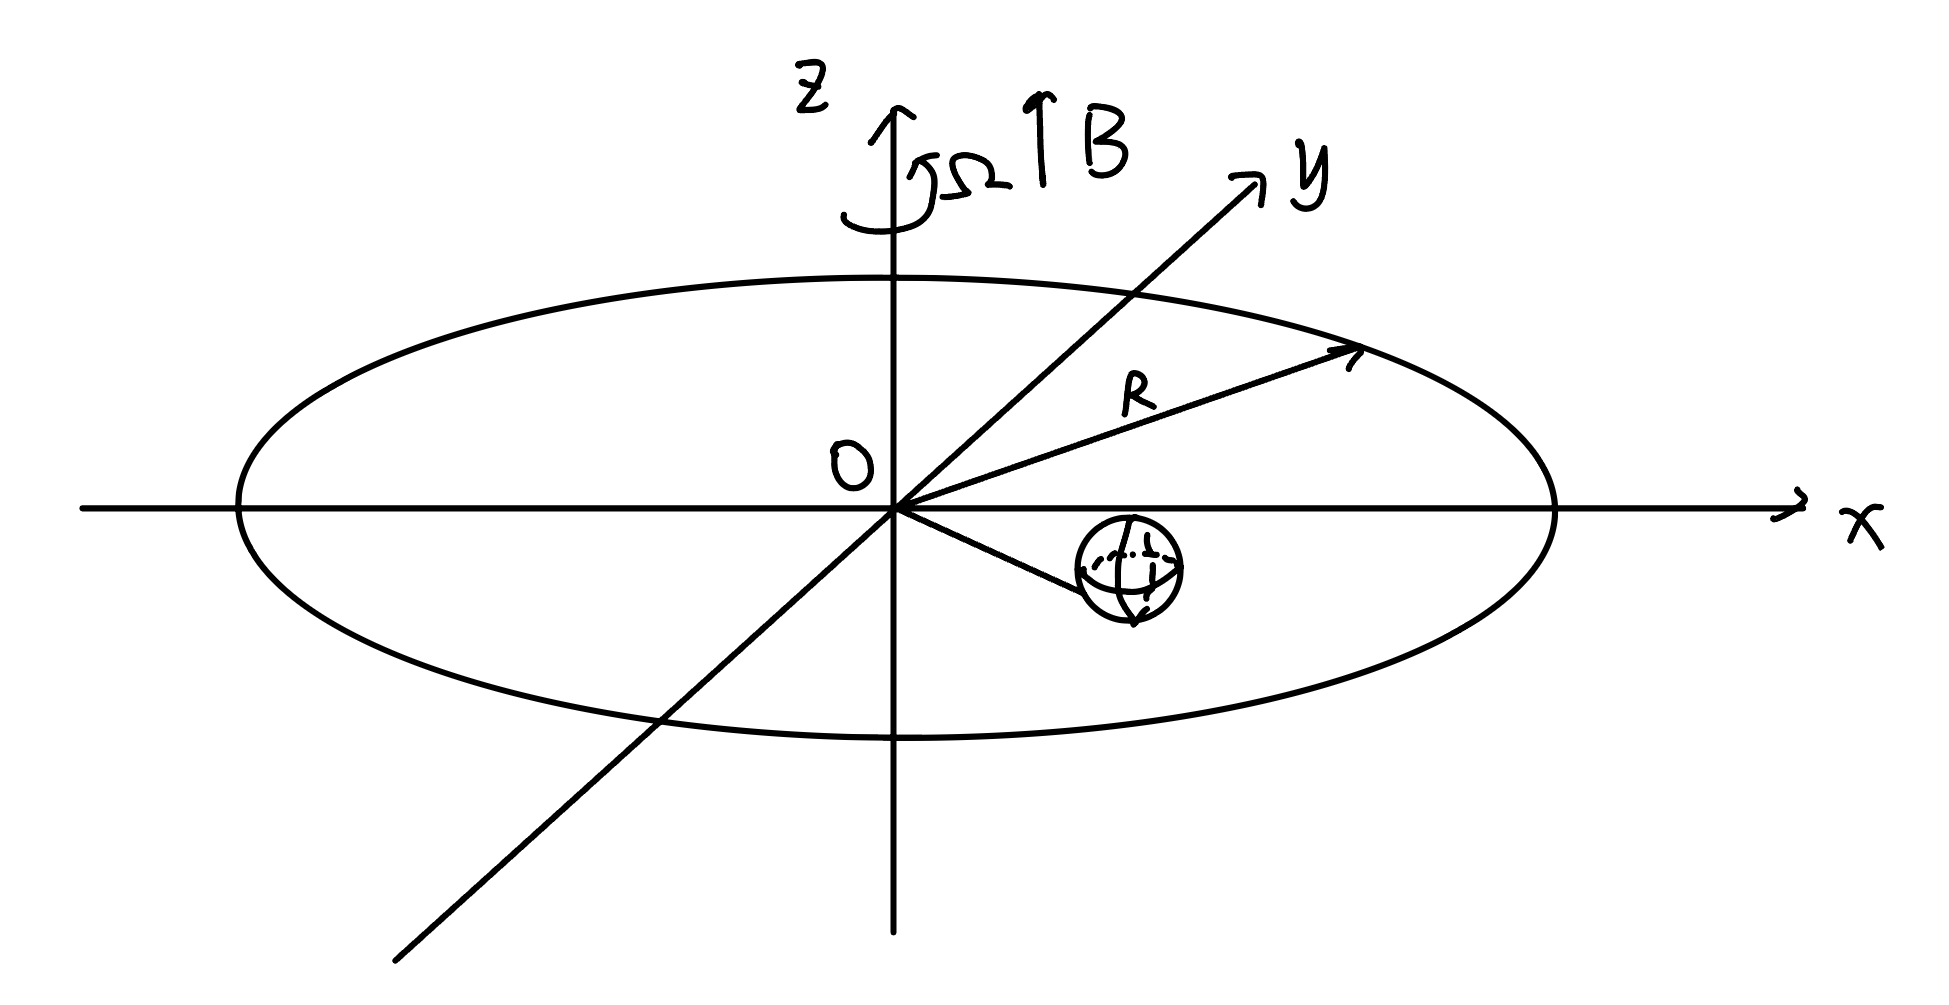
\includegraphics[width=4cm]{img/1.jpeg}\\
	\vspace{-15pt}    % 对应高度2
	\caption{}
	\vspace{-15pt}    % 对应高度3
\end{wrapfigure}
光滑水平面上有一木块,匀质质量为$M$,在左端中间固定有一档板,其上有一绳,一侧系有一质量为$m$得质点。其中各参数如图所示,初态均静止,细绳水平释放质点。
试就$\frac{M}{m}=1,\frac{1}{2}$时,求木块右侧是否会离开地面。若会,其第一次离开时的$\theta$ .
\end{document}